\documentclass{article}\usepackage[]{graphicx}\usepackage[]{color}
%% maxwidth is the original width if it is less than linewidth
%% otherwise use linewidth (to make sure the graphics do not exceed the margin)
\makeatletter
\def\maxwidth{ %
  \ifdim\Gin@nat@width>\linewidth
    \linewidth
  \else
    \Gin@nat@width
  \fi
}
\makeatother

\definecolor{fgcolor}{rgb}{0.345, 0.345, 0.345}
\newcommand{\hlnum}[1]{\textcolor[rgb]{0.686,0.059,0.569}{#1}}%
\newcommand{\hlstr}[1]{\textcolor[rgb]{0.192,0.494,0.8}{#1}}%
\newcommand{\hlcom}[1]{\textcolor[rgb]{0.678,0.584,0.686}{\textit{#1}}}%
\newcommand{\hlopt}[1]{\textcolor[rgb]{0,0,0}{#1}}%
\newcommand{\hlstd}[1]{\textcolor[rgb]{0.345,0.345,0.345}{#1}}%
\newcommand{\hlkwa}[1]{\textcolor[rgb]{0.161,0.373,0.58}{\textbf{#1}}}%
\newcommand{\hlkwb}[1]{\textcolor[rgb]{0.69,0.353,0.396}{#1}}%
\newcommand{\hlkwc}[1]{\textcolor[rgb]{0.333,0.667,0.333}{#1}}%
\newcommand{\hlkwd}[1]{\textcolor[rgb]{0.737,0.353,0.396}{\textbf{#1}}}%

\usepackage{framed}
\usepackage{graphicx}

\usepackage[utf8]{inputenc}
 
\usepackage{listings}
\usepackage{color}
 
\definecolor{codegreen}{rgb}{0,0.6,0}
\definecolor{codegray}{rgb}{0.5,0.5,0.5}
\definecolor{codepurple}{rgb}{0.58,0,0.82}
\definecolor{backcolour}{rgb}{0.95,0.95,0.92}
 
\lstdefinestyle{mystyle}{
    backgroundcolor=\color{backcolour},   
    commentstyle=\color{codegreen},
    keywordstyle=\color{magenta},
    numberstyle=\tiny\color{codegray},
    stringstyle=\color{codepurple},
    basicstyle=\footnotesize,
    breakatwhitespace=false,         
    breaklines=true,                 
    captionpos=b,                    
    keepspaces=true,                 
    numbers=left,                    
    numbersep=5pt,                  
    showspaces=false,                
    showstringspaces=false,
    showtabs=false,                  
    tabsize=2
}
 
\lstset{style=mystyle}
 

\makeatletter
\newenvironment{kframe}{%
 \def\at@end@of@kframe{}%
 \ifinner\ifhmode%
  \def\at@end@of@kframe{\end{minipage}}%
  \begin{minipage}{\columnwidth}%
 \fi\fi%
 \def\FrameCommand##1{\hskip\@totalleftmargin \hskip-\fboxsep
 \colorbox{shadecolor}{##1}\hskip-\fboxsep
     % There is no \\@totalrightmargin, so:
     \hskip-\linewidth \hskip-\@totalleftmargin \hskip\columnwidth}%
 \MakeFramed {\advance\hsize-\width
   \@totalleftmargin\z@ \linewidth\hsize
   \@setminipage}}%
 {\par\unskip\endMakeFramed%
 \at@end@of@kframe}
\makeatother

\definecolor{shadecolor}{rgb}{.97, .97, .97}
\definecolor{messagecolor}{rgb}{0, 0, 0}
\definecolor{warningcolor}{rgb}{1, 0, 1}
\definecolor{errorcolor}{rgb}{1, 0, 0}
\newenvironment{knitrout}{}{} % an empty environment to be redefined in TeX

\usepackage{alltt} % For LaTeX2e

% Set to togglefalse to use nips formatting.
% Set to toggletrue to use arxiv formatting.
\usepackage{etoolbox}
\newtoggle{arxivformat}
\toggletrue{arxivformat}
%\togglefalse{arxivformat}

\iftoggle{arxivformat} {
  \usepackage[sort&compress, numbers]{natbib}
  \usepackage{times}
}{
  \usepackage{nips15submit_e,times}
  \usepackage[sort&compress, numbers]{natbib}
}

\usepackage{hyperref}
%\usepackage{url}
%\documentstyle[nips14submit_09,times,art10]{article} % For LaTeX 2.09

\usepackage[margin=1.5in]{geometry}

\usepackage{graphicx} % more modern
\usepackage{subcaption}
\usepackage{caption}

\usepackage{amsthm}
\usepackage{amsmath}
\usepackage{appendix}

\usepackage{placeins}

\let\Oldsection\section
\renewcommand{\section}{\FloatBarrier\Oldsection}

\let\Oldsubsection\subsection
\renewcommand{\subsection}{\FloatBarrier\Oldsubsection}

\let\Oldsubsubsection\subsubsection
\renewcommand{\subsubsection}{\FloatBarrier\Oldsubsubsection}

% Do not break equations across pages
%\allowdisplaybreaks

% Used to number single equations in an equation array.
\newcommand\numberthis{\addtocounter{equation}{1}\tag{\theequation}}

\usepackage{amssymb}
\usepackage{bbm}

% references
\newcommand{\app}[1]{Appendix~\ref{app:#1}}
\newcommand{\lem}[1]{Lemma~\ref{lem:#1}}
\newcommand{\prop}[1]{Proposition~\ref{prop:#1}}
\newcommand{\rem}[1]{Remark~\ref{rem:#1}}
\newcommand{\mysec}[1]{Section~\ref{sec:#1}}
\newcommand{\mysecs}[1]{Sections~\ref{sec:#1}}
\newcommand{\mysecss}[1]{\ref{sec:#1}}
\newcommand{\eq}[1]{Eq.~(\ref{eq:#1})}
\newcommand{\eqs}[1]{Eqs.~(\ref{eq:#1})}
\newcommand{\eqss}[1]{(\ref{eq:#1})}
\newcommand{\eqw}[1]{Eq.~(#1)}
\newcommand{\fig}[1]{Fig.~(\ref{fig:#1})}
\newcommand{\figs}[1]{Figs.~(\ref{fig:#1})}
\newcommand{\figss}[1]{(\ref{fig:#1})}

% macros
\newcommand{\npp}{\tilde{\eta}} % natural parameter for the p distribution
\newcommand{\npq}{\eta} % natural parameter for the q distribution
\newcommand{\mpp}{\tilde{m}} % mean parameter for the p distribution
\newcommand{\mpq}{m} % mean parameter for the q distribution
\newcommand{\mpopt}{m^*} % mean parameter for the q^* distribution
\newcommand{\npopt}{\eta^*} % mean parameter for the q^* distribution
\newcommand{\gauss}{\mathcal{N}} % Gaussian distribution
\newcommand{\truecov}{\Sigma} % True posterior covariance
\newcommand{\lrcov}{\hat{\Sigma}} % LR cov estimate
\newcommand{\vbcov}{V} % Variational posterior covariance
\newcommand{\constant}{C} % A constant
\newcommand{\klshort}{E}

% theorems
\theoremstyle{plain}
\newtheorem{theorem}{Theorem}[section]

\newtheorem{proposition}[theorem]{Proposition}
\newtheorem{lemma}[theorem]{Lemma}
\newtheorem{remark}[theorem]{Remark}

% other macros
\newcommand{\kl}{\textrm{KL}}
\DeclareMathOperator*{\argmin}{arg\,min}
\DeclareMathOperator*{\argmax}{arg\,max}
\newcommand{\mbe}{\mathbb{E}}
\newcommand{\mbeq}{\mathbb{E}_{q}}
\newcommand{\var}{\textrm{Var}}
\newcommand{\cov}{\textrm{Cov}}
\newcommand{\iid}{\stackrel{iid}{\sim}}
\newcommand{\indep}{\stackrel{indep}{\sim}}

\title{Reinforcement Learning : Dynamic Programming\\
Technical Report}

% To keep the emails from being too big
\usepackage[scaled=0.7]{beramono}

% TODO: fix these citations.
\author{
Riashat Islam\\
%Department of Statistics\\
McGill University\\
Reasoning and Learning Lab\\
%Berkeley, CA 94720 \\
\texttt{riashat.islam@cs.mcgill.ca}
}

\newcommand{\fix}{\marginpar{FIX}}
\newcommand{\new}{\marginpar{NEW}}

\iftoggle{arxivformat} {
}{
  \nipsfinalcopy % Uncomment for camera-ready version
}
\IfFileExists{upquote.sty}{\usepackage{upquote}}{}
\begin{document}

\maketitle










\section{Introduction}

\noindent
In this work, we consider analysis of the basic reinforcement learning algorithms such as value iteration and policy iteration on three different models, namely smallworld, gridworld and cliffworld MDPs. We consider value and policy iteration and discuss the proof of convergence for these algorithms. We implemented value and policy iteration algorithms in matlab, and demonstrated its effectiveness in converging to an optimal value function and policy. We also include an interpretation of how policy iteration can be considered to be similar to Newton's method.



\subsection{Experimental Setup}

\noindent
\noindent
\textbf{Models/Environments}: We consider experiments over three different benchmark RL tasks. For all the environments, the agent is allowed $4$ discrete actions in a discrete state space. In the Small World MDP (model), the goal states (state with maximal reward) is at the coordinates $(4,4)$. We consider a constant reward of $-1$ in all the states, reward of $10$ in the goal state and a negative reward (cost) of $-6$ in the bad state. The smallworld MDP has $17$ different states. Similarly, the gridworld MDP has $109$ different states, with the goal state at $93$ and pre-defined start state. We also consider a cliffworld MDP with the usual actions of up, down, left and right, with a reward of $-1$ for all transitions, except for a reward of $-100$ if the agent enters the cliff, and a reward of $10$ in the goal state with co-ordinates $(5,9)$. We always consider discounted MDPs with $\gamma=0.9$. Our work also considers careful fine-tuning of the $\epsilon$ parameter for greedy action selection as discussed later. We always consider stochastic discrete policies in a model-based environment with given transition dynamics. 









\section{Value Iteration}

\noindent
In reinforcement learning, value iteration concerns with finding the optimal policy $\pi$ using an iterative application of the Bellman optimality backup. At each iteration, value iteration uses synchronous updates for all the states to update the value function, ie, update $V_{k+1}(s)$ from $V_k(s')$.  In our work, we consider using value iteration over the gridworld model. In order for value iteration to converge, it requires an infinite number of iterations to converge to $V*$. We use the stopping criterion for value iteration that when there are no further improvements to the value function, or when the change in value function is less than a very small positive number in a given sweep, we terminate the algorithm. Value iteration is guaranteed to converge to an optimal policy for finite MDPs with a discounted reward. Unlike policy iteration, there is no explicit policy in value iteration. In our algorithm, we evaluate the policy at each step of the episode as shown by the code below.

\begin{equation}
    V_{k+1}(s) = \max_{a \in A} (R_s^{a} + \gamma (\sum_{s' \in S} P_{ss'}^{a} V_{k}(s'))
\end{equation}


\noindent
We include a brief snippet of our value iteration algorithm implementation as below:


\begin{lstlisting}[language=Matlab, caption=Value Iteration Algorithm]
% run VI on GridWorld
gridworld;
[v, pi] = valueIteration(model, 1000)
plotVP(v,pi, paramSet)

%value iteration algorithm
function [v, pi] = valueIteration(model, maxit)
% initialize the value function
v = zeros(model.stateCount, 1);
pi = ones(model.stateCount, 1);
old_v = zeros(model.stateCount, 1);
threshold =  1.0000e-22;

for iterations = 1:maxit,
    % initialize the policy and the new value function
    policy = ones(model.stateCount, 1);
    v_ = zeros(model.stateCount, 1);
    % perform the Bellman update for each state
    for s = 1:model.stateCount,
    %compute transition probability
    P = reshape(model.P(s,:,:), model.stateCount, 4);  
    %update value function
    [v_(s,:), action] = max(model.R(s,:) + 
        (model.gamma * P' * v)');
    %policy evaluated every step
    policy(s,:) = action;        
    end   
old_v = v;    
v = v_;
pi = policy; 
%break condition
%to check convergence of VI algorithm
if v - old_v <= threshold
    fprintf('Value function converged 
    after \%d iterations\n',iterations);
        break;
end      

end
end


\end{lstlisting}





\subsection{Experimental Results}
\noindent
We demonstrate the effectiveness of value iteration algorithm on three model environments, namely smallworld, gridworld and cliffworld. First we show the performance of our value iteration algorithm on a 2D grid, where lighter region indicates a better learnt policy at that state, compared to the darker regions. The cumulative reward of 0 indicates the maximum reward that can be achieved. We basically used negative rewards, where a large negative cumulative reward would indicate the agent performing poorly.\\

\noindent
Value iteration algorithm on small world MDP with 100 and 1000 iterations as shown in figure \ref{figure1} and \ref{figure2} below:

 



\begin{figure}[h!]
  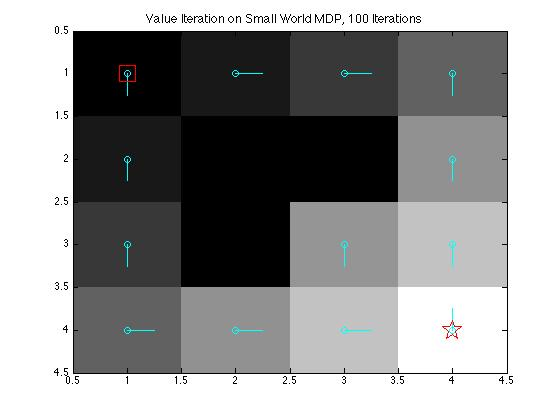
\includegraphics[scale=0.5]{Value100.jpg}
  \caption{Value iteration on Small World MDP with 100 iterations}
  \label{figure1}
\end{figure}


\begin{figure}[h!]
  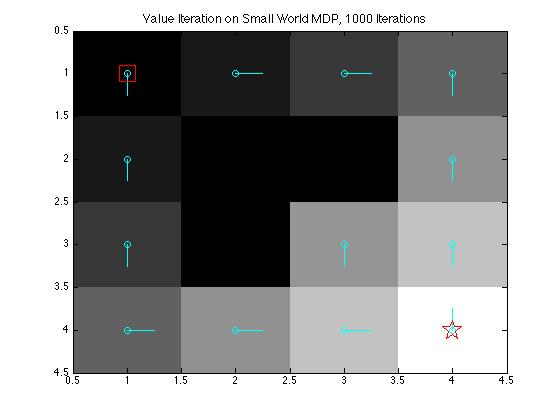
\includegraphics[scale=0.5]{Value1000.jpg}
  \caption{Value iteration on Small World MDP with 1000 iterations}
  \label{figure2}
\end{figure}





\noindent
The results above indicate that the learnt value function is the same for both 100 and 1000 iterations. This means that for the smallworld MDP case, the value iteration algorithm converges really fast, especially since it is a small environment we are considering here. This can be further demonstrated by plotting the cumulative reward plot for both 100 and 1000 iterations. Results show that the maximum cumulative reward achieved, or in other words the value function converges within 50 iterations in the smallworld MDP case.\\


\begin{figure}[h!]
  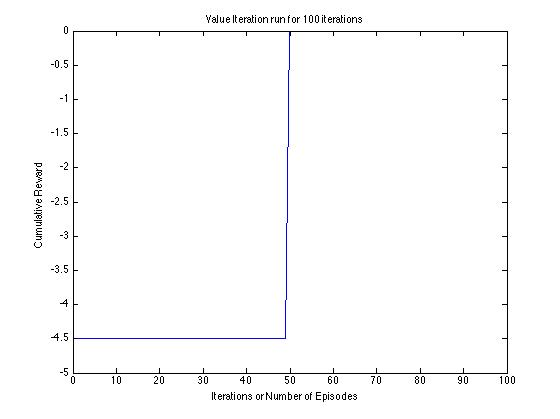
\includegraphics[scale=0.5]{value100_CumRwd.jpg}
  \caption{Cumulative reward of agent following value iteration on Small World MDP with 100 iterations}
  \label{figure3}
\end{figure}


\begin{figure}[h!]
  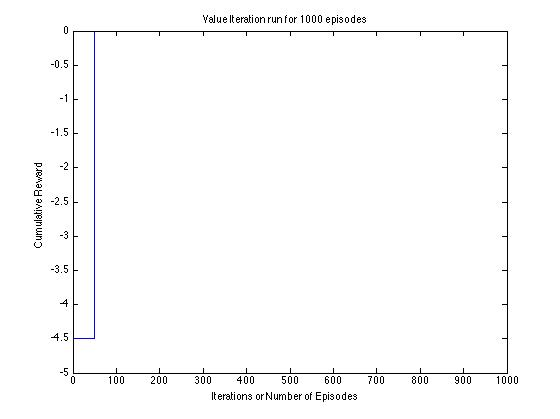
\includegraphics[scale=0.5]{value1000_CumRwd.jpg}
  \caption{Cumulative reward of agent following value iteration on Small World MDP with 1000 iterations}
  \label{figure4}
\end{figure}

 
 


\noindent
In a similar way, we can evaluate the performance of our value iteration algorithm on the gridworld and cliffworld MDPs, which are much larger environments, as shown in figures \ref{figure5} and figure \ref{figure6} below. We ran our value iteration algorithm for 1000 episodes for both MDPs.\\



\begin{figure}[h!]
  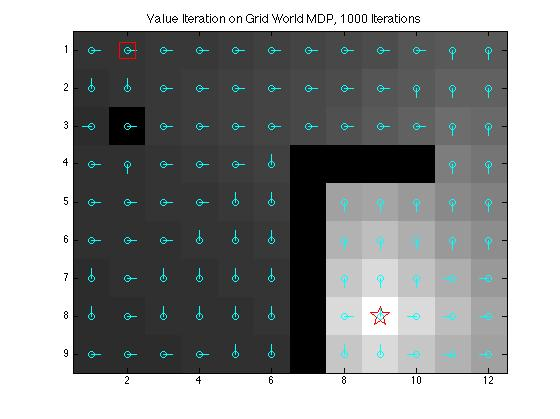
\includegraphics[scale=0.5]{value1000_GridWorld.jpg}
  \caption{Value Iteration on Grid World MDP with 1000 iterations}
  \label{figure5}
\end{figure}


\begin{figure}[h!]
  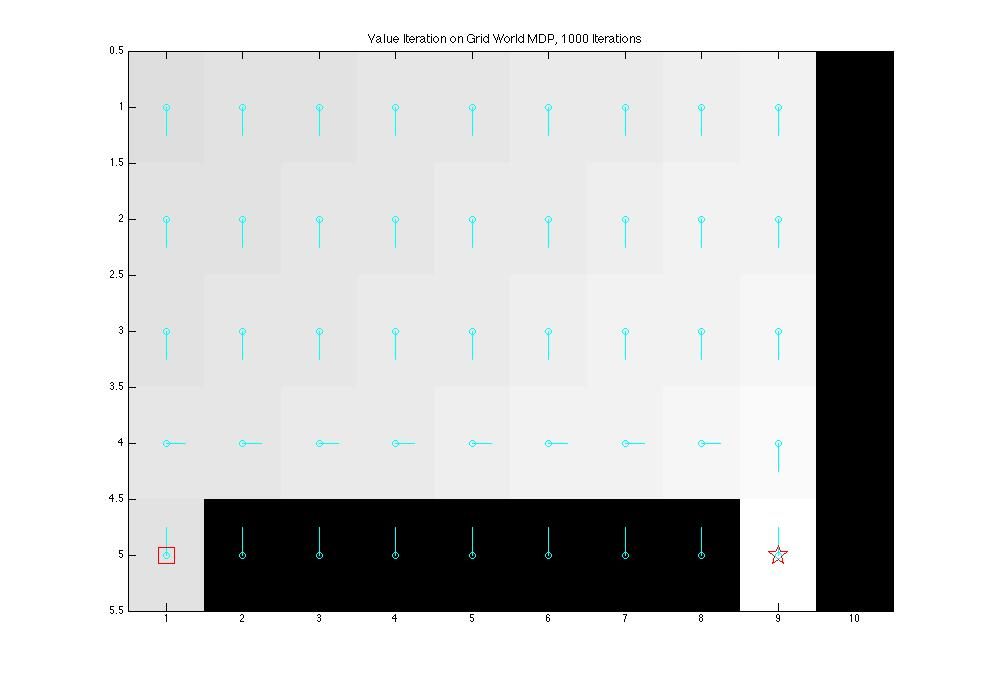
\includegraphics[scale=0.4]{value1000_Cliffworld.jpg}
  \caption{Value Iteration on Cliff World MDP with 1000 iterations}
  \label{figure6}
\end{figure}








\noindent
\textit{Testing for convergence of Value Iteration on different environments : } In order to check for convergence of value iteration and how it depends on the state space of the environment, we ran the algorithm for same number of iterations on the different environments. Figure \ref{figure7} summarizes how the convergence of value iteration algorithm depends on the size of the environment. For convenice, we only show the plot for upto 500 iterations since the algorithm converges within that number of iterations.

\begin{figure}[h!]
  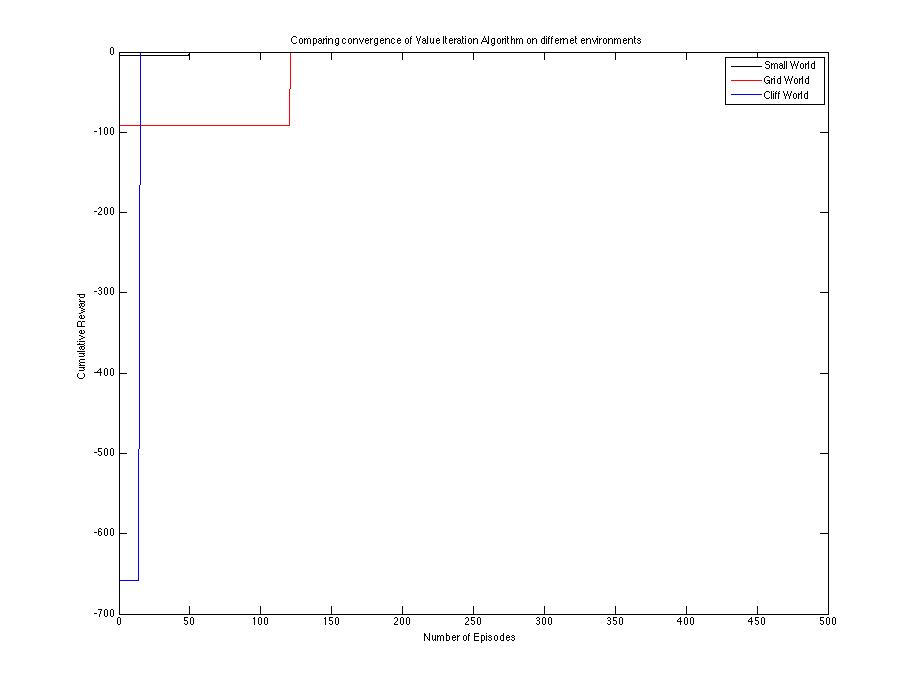
\includegraphics[scale=0.4]{comparison.jpg}
  \caption{Comparison of convergence of value iteration on different environments}
  \label{figure7}
\end{figure}
















\section{Policy Iteration}

\noindent
We then consider policy iteration instead of value iteration on the gridworld model. Policy iteration uses an iterative policy evaluation step to estimate $V^{\pi}$ and a policy improvement step to generate $\pi' > \pi$, where $\pi'$ is obtained by a greedy policy improvement step. The policy evaluation step evaluates the value function for a given policy $\pi$ using an iterative Bellman expectation backup. The policy improvement step is then the action that maximizes the value function, using a greedy policy improvement step. In other words, policy iteration obtains a sequence of continually improving policies and value functions, where we do policy evaluation and improvement separately, while every policy improvement is guaranteed to be an improvement. 




\subsection{Experimental Results}

\noindent
We then implemented the policy iteration algorithms on the same environments, and evaluated the convergence of this algorithm. Figures \ref{figure8}, \ref{figure9} and \ref{figure10} shows the policy iteration algorithm on smallworld, gridworld and cliffworld MDPs. Similar to above, we again ran the policy iteration algorithm with 1000 iterations. The results show that similar plots are obtained for value iteration as for policy iteration, suggesting that the algorithm converges similar to value iteration.\\


\noindent
Below we include a brief code snippet of out implementation of the policy iteration algorithm.


\begin{lstlisting}[language=Matlab, caption=Policy Iteration Algorithm]
function [v, pi] = policyIteration(model, maxit)

% initialize the value function
v = zeros(model.stateCount, 1);
pi = ones(model.stateCount, 1);
% old_v = zeros(model.stateCount, 1);
policy = ones(model.stateCount, 1);
tol = 0.0000000000000000000001;

%run this extra loop
% to check for convergence 
%in policy evaluation and 
%policy improvement step
for iterations = 1:maxit,
     
    % Policy Evaluation Step
    %with same number of episodes
    for i = 1:maxit,
    v_ = zeros(model.stateCount, 1);
    % perform the Bellman update for each state
    for s = 1:model.stateCount
    v_(s) = model.R(s, policy(s)) 
    + (model.gamma*model.P(s,:,policy(s))*v)';
    end          
    delta = norm(v - v_);
    v = v_;
    
%check for convergence
if delta <= tol
fprintf('Value function 
converged after $\%$ d iterations\n',i);
break;
end     
end    

for s = 1:model.stateCount    
    P =reshape(model.P(s,:,:),model.stateCount,4);    
    [~, action] = 
    max(model.R(s,:) + (model.gamma *P'*v)');
        
    policy(s) = action;
end
end
pi = policy;
v = v_;

end


\end{lstlisting}








\begin{figure}[h!]
  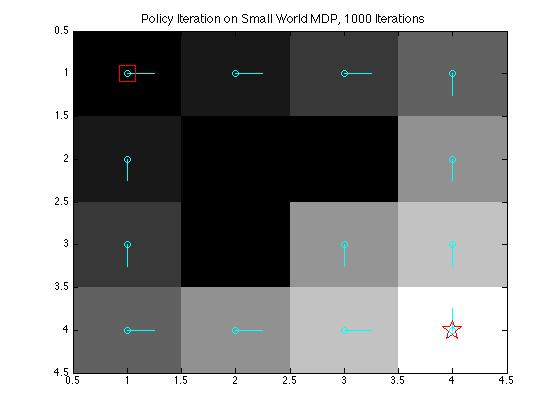
\includegraphics[scale=0.5]{policy1000_small.jpg}
  \caption{Policy iteration on small world MDP with 1000 iterations}
  \label{figure8}
\end{figure}



\begin{figure}[h!]
  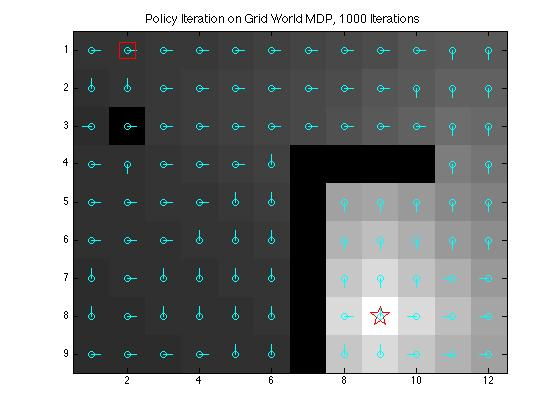
\includegraphics[scale=0.5]{policy1000_grid.jpg}
  \caption{Policy iteration on grid world MDP with 1000 iterations}
  \label{figure9}
\end{figure}


\begin{figure}[h!]
  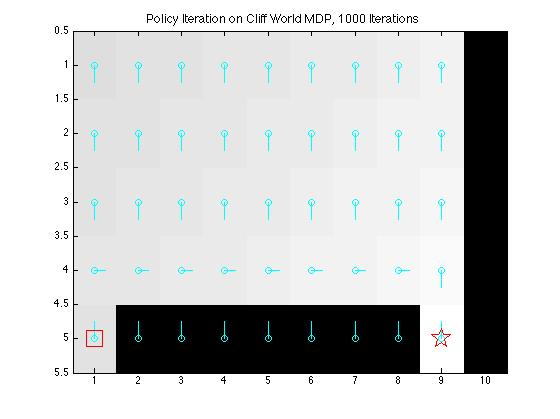
\includegraphics[scale=0.5]{policy1000_cliff.jpg}
  \caption{Policy iteration on cliff world MDP with 1000 iterations}
  \label{figure10}
\end{figure}





\noindent
However, we note that the policy iteration algorithm takes longer to run than the value iteration algorithm. This is mainly because we first test for convergence of the value function, after which there is a greedy maximisation step to improve the policy. Due to two loops in the algorithm, one for converging value function - the policy evaluation step, and one for improving the policy - the policy improvement step - the policy iteration algorithm takes longer to converge. 






\section{Convergence of Value and Policy Iteration}


\noindent
Our insight is that,  the policy iteration algorithm takes longer to run and takes longer time for convergence than the value iteration algorithm. The speed of convergence is faster for value iteration compared to policy iteration. Here are some reasons why\\


\noindent
The value iteration algorithm converges after 88 iterations. Compared to that, the policy iteration algorithm converges after 120 iterations. This further validates that using value iteration, we can converge faster to the optimal policy $\pi^{*}$. The reason is further explained below:\\

\noindent
A usefulness of value iteration algorithm is that it takes smaller time to converge since it is independent of the actual policy. We are directly optimising the value function. Compared to that, in policy iteration, there are two steps of policy evaluation and policy improvement. The policy iteration algorithm first checks for convergence of value function under the given policy. Then it tries to improve the policy under the given value function, and the process repeats. Until an improved policy gives a better value function, which in turn would give the same policy at the policy improvement step, the policy iteration algorithm is not guaranteed to converge. The two loops in the algorithm makes policy iteration algorithm slower in terms of convergence. However, both the algorithms are guaranteed to converge to the optimal policy given it is ran for large number of times.










\section{Theoretic Analysis of Convergence of Policy Iteration}

\noindent
In this section, we include a brief theoretical analysis of the proof of convergence of the policy iteration algorithm.\\



\noindent
This section considers the proof of convergence of the policy iteration algorithm. We denote our policy as $\pi(s)$ and the Bellman operator as $T$.  As discussed earlier, policy iteration algorithm involves two steps: policy improvement followed by policy evaluation.\\

\noindent
First we show that by acting greedily means policy improvement $\pi'(s) > \pi(s)$ for every greedy action. Since the value function is given as $V_{\pi(s)} = R_s + \gamma P^{\pi} V $, greedy action means:

\begin{equation}
    \pi'(s) = \arg \max_a [R_s + P^{\pi} V]
\end{equation}

\noindent
therefore, a greedy action leads to an improvement in the value function:

\begin{equation}
    V_{\pi'(s)} \geq V_{\pi(s)}
\end{equation}

\noindent
In other words, since $Q_{\pi} (s, \pi(s)) = V_{\pi} (s)$, this means

\begin{equation}
    Q_{\pi} (s, \pi'(s)) \geq Q_{\pi} (s, \pi(s))
\end{equation}


\noindent
We can therefore prove that a policy improvement step in the policy iteration algorithm leads to $V_{\pi'} (s)\geq V_{\pi} (s)$ as follows:
\noindent
\begin{equation}\label{improvement_proof}
    \begin{split}
    
        V_{\pi}(s) & = \leq Q_{\pi} (s, \pi'(s))
        
        & = E_{\pi} [R_{t+1} + \gamma V_{\pi} (s_{t+1}) | s_t ]
        
        & = \leq E_{\pi'} [R_{t+1} + \gamma Q_{\pi} (s_{t+1}, \pi'(s_{t+1})) | s_t ]
        
        & = \leq E_{\pi'} [R_{t+1} + \gamma R_{t+2} + \gamma^2 Q_{\pi} (s_{t+2}, \pi'(s_{t+2})) | s_t
        
        & = \leq E_{\pi'} [R_{t+1} + \gamma R_{t+2} + ... | s_t]
        
        & = V_{\pi'} (s)
        
        
    \end{split}
\end{equation}


\noindent
The policy improvement step in policy iteration therefore guarantees that:

\begin{equation}
    V^{\pi_{k+1}} \geq V^{\pi_k}
\end{equation}

\noindent
Using the Bellman operator this therefore means:


\noindent
\begin{equation} \label{eq1}
\begin{split}

V^{\pi_k} & = T^{\pi_k} V^{\pi_k} 

V^{\pi_k} & = \leq T V^{\pi_k} 

V^{\pi_k} & = T^{\pi_{k+1}} V^{\pi_k} 

\end{split}
\end{equation}

\noindent
where $ \pi_{k+1} $ is an improved policy following greedy policy improvement. We want to show that following each step of policy improvement, there is an improvement in the value function given by the Bellman operator as follows:


\begin{equation}
    V^{\pi_k} \leq T^{\pi_{k+1}} V^{\pi_k} 
\end{equation}


\noindent
Hence, following the Bellman operator, the improvement of policy from $\pi_k$ to $\pi_{k+1}$ shows an improvement in the value function as given by:


\begin{equation}
    V^{\pi_k} \leq T^{\pi_{k+1}} V^{\pi_k} \leq ( T^{\pi_{k+1}} )^{2} V^{\pi_k} \leq ...
\end{equation}


\noindent
Hence, we can show that:

\begin{equation}
    V^{\pi_k} \leq lim_{n -> \inf} ( T^{\pi_{k+1}} )^{n} V^{\pi+k} = V^{\pi_{k+1}}
\end{equation}


\noindent
Following iterations in policy iteration algorithm, when the policy improvement stops, ie $\pi'(s) = \pi(s) $, or alternatively we can write $Q_{\pi} (s, \pi'(s)) = Q_{\pi} (s, \pi(s)) = V_{\pi} (s) $. When an optimal policy is reached following greedy policy improvement steps, it will satisfy the Bellman optimality equation:

\begin{equation}
\label{optimal}
    V^{\pi_k} = V^{*}
\end{equation}

\noindent
So the algorithm stops after finite steps k, when there is no more improvement in policy improvement step, and hence the policy evaluation step. 
\noindent
\textbf{This means convergence of the policy iteration algorithm is guaranteed}. Policy iteration stops when there are no more improvements by taking a greedy action, and the Bellman optimality equation is satisfied as given by equation \ref{optimal}.\\


\noindent
\textbf{There exists only a finite number of policies in a given MDP}. However, there exists only one optimal deterministic policy for any setting. Since the number of policies is finite, so the policy iteration algorithm steps must also converge after a finite k steps as:

\begin{equation}
    V^{\pi_{q}} = V^{\pi_{q+1}}
\end{equation}


\noindent
$V^{\pi_{q}}$ is a fixed point of T, and since T has a unique fixed point, we can therefore also deduce that:

\begin{equation}
    V^{\pi_q} = V^{*} 
\end{equation}

\noindent
and hence $\pi_q$ is an optimal policy. 
















\section{Policy Iteration as Newton's Method}

\noindent
We will include a brief intuitive understanding of how policy iteration can be considered similar to Newton's method. Similar to Newton's method, the policy evaluation step can be considered as deriving the value of $f(x)$ for a given x, just as we would derive the value function as an expected sum of rewards. Thereafter, since the policy iteration has a step involving maximisation of the value function to find an action that would maximise the value - this can be considered the same as finding the gradient and updating $x$ in $f(x)$ in the direction of the gradient. The update in the point $x$ in $f(x)$ by finding the gradient of the function is similar to the policy improvement step where the maximisation essentially chooses an action that would increase the value function.\\





\section{Conclusion}

\noindent
In this report, we included basic implementations of the value and policy iteration algorithms, and demonstrated their performances on three different environments. For all the environments, we showed the convergence of the policy and value iteration algorithms to the optimal policy. We also discussed that even though the policy iteration algorithm may take longer time to compute and it has a lower speed of convergence mainly because the policy improvement step chooses actions which would maximise the value function. Hence, even if considering the contraction mapping theorem, the value function would converge to an optimal value function much faster. We then briefly demonstrated theoretical guarantees of the convergence of policy iteration, which is in line with what has been shown in the demonstrated experiments. Finally, we included an intuitive interpretation of how the policy iteration algorithm can be considered to be similar to Newton's method. 



\end{document}